\documentclass[glossy]{beamer}
\useoutertheme{wuerzburg}
\useinnertheme[realshadow,corners=2pt,padding=2pt]{chamfered}
\usecolortheme{shark}
\usepackage[utf8]{inputenc} % codificacao de caracteres
\usepackage[T1]{fontenc}    % codificacao de fontes
\usepackage[brazil]{babel}
\usepackage{graphicx} % Allows including images
\usepackage{booktabs} % Allows the use of \toprule, \midrule and \bottomrule in tables
\usepackage[absolute,overlay]{textpos}
\usepackage{movie15}
\usepackage{verbatim}

\usepackage{tikz}
\newcommand<>{\hover}[1]{\uncover#2{%
 \begin{tikzpicture}[remember picture,overlay]%
 \draw[fill,opacity=0.4] (current page.south west)
 rectangle (current page.north east);
 \node at (current page.center) {#1};
 \end{tikzpicture}}
}

\title{Integração Contínua, Entrega Contínua e Implantação Contínua (CI \& CD)}
\author{Lucas Fonseca, Marco Aurélio}
\institute{Universidade Federal de Lavras}
\date{28 de junho de 2019}

\begin{document}

\begin{frame}
\maketitle
\end{frame}

\begin{comment}
    \begin{textblock*}{5cm}(9cm,7cm) % {block width} (coords)
    \includegraphics[scale=0.3]{no-sql.png}
    \end{textblock*}
\end{comment}

\begin{frame}

\frametitle{Conteúdo} % Table of contents slide, comment this block out to remove it
\tableofcontents % Throughout your presentation, if you choose to use \section{} and \subsection{} commands, these will automatically be printed on this slide as an overview of your presentation
\end{frame}

\section{Introdução}
    \begin{frame}{Introdução}
    \begin{itemize}
        \item Competitividade;
        \item Gerar Valor Rápido;
        \item Metodologias Ágeis;
        \item Cultura DevOps;
        \item Cloud Computing;
    \end{itemize}
    
    \begin{textblock*}{5cm}(7cm,2cm) % {block width} (coords)
        
\includegraphics[scale=0.18]{img/scrum-logo.png}
    \end{textblock*}
    
    \begin{textblock*}{5cm}(5cm,1.3cm) % {block width} (coords)
        
\includegraphics[scale=0.111]{img/valor.png}
    \end{textblock*}
    
    \begin{textblock*}{5cm}(6cm,4.5cm) % {block width} (coords)
        
\includegraphics[scale=0.16]{img/devops2.png}
    \end{textblock*}
    
    \begin{textblock*}{5cm}(1cm,7cm) % {block width} (coords)
        
\includegraphics[scale=0.18]{img/aws.png}
    \end{textblock*}
    
    \begin{textblock*}{5cm}(4cm,6.7cm) % {block width} (coords)
        
\includegraphics[scale=0.1]{img/gcp.png}
    \end{textblock*}
    
    \begin{textblock*}{5cm}(8cm,7cm) % {block width} (coords)
        
\includegraphics[scale=0.08]{img/azure.png}
    \end{textblock*}
    \end{frame}

\section{Cultura DevOps}
    \begin{frame}{Cultura DevOps}
    \begin{figure}[h]
        \centering
        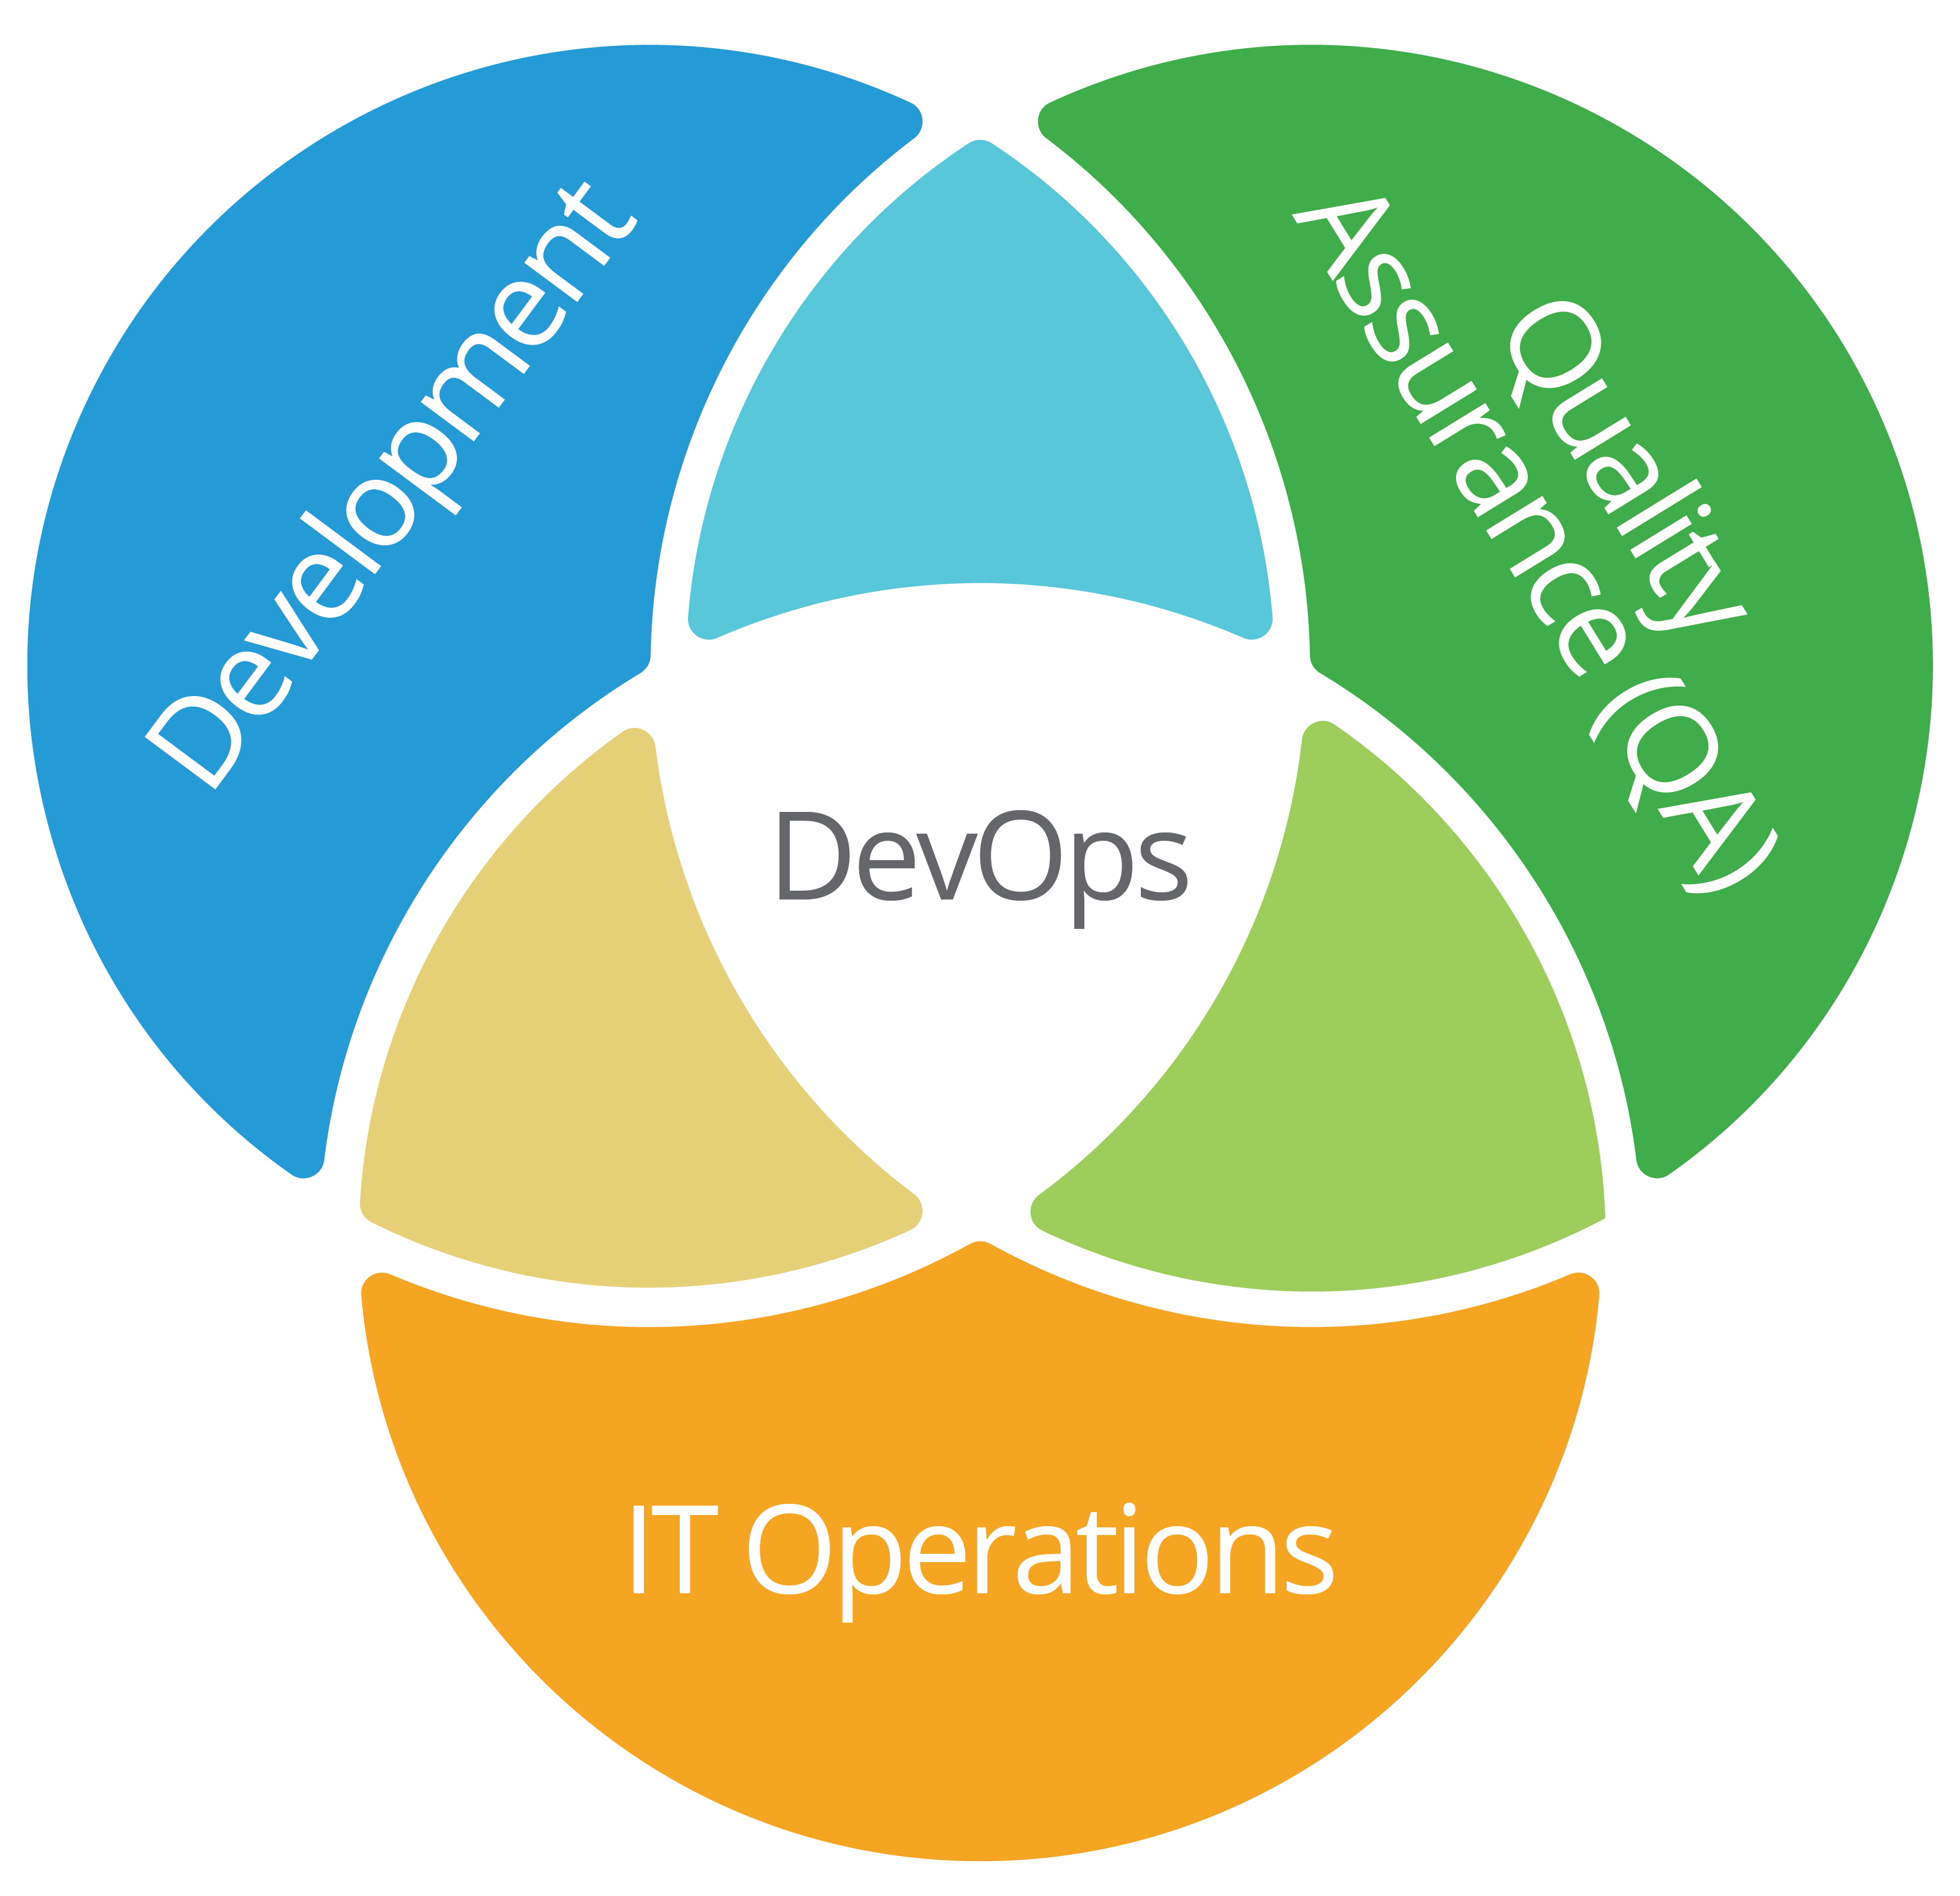
\includegraphics[scale=0.26]{img/devops.jpg}
    \end{figure}    
    \end{frame}

\section{Integração Contínua}
    \begin{frame}{Integração Contínua (Continuous Integration)}
    \begin{itemize}
        \item Prática de desenvolvimento;
        \item Integrar o código frequentemente;
        \item Pelo menos uma vez por dia;
        \item Servidor de CI;
        \item Build automática;
        \item Testes automatizados;
        \item Validar o código;
        \item Código sempre em estado deployable;
    \end{itemize}
    \end{frame}
    
    \begin{frame}{Integração Contínua (Continuous Integration)}
    \begin{figure}[h]
        \centering
        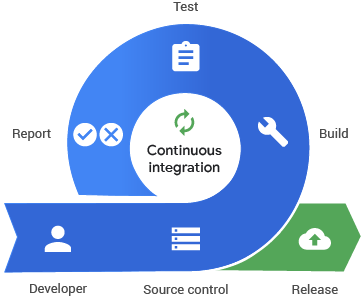
\includegraphics[scale=0.6]{img/ci.png}
    \end{figure}    
    \end{frame}

\section{Vantagens da Integração Contínua}
    \begin{frame}{Por Que Implementar Integração Contínua?}
        \begin{itemize}
            \item Evita conflitos de código ao realizar o merge;
            \item Detecção rápida de erros;
            \item Evitar bugs em produção;
            \item Muito mais fácil corrigir erros;
            \item Promove comunicação humana quando um conflito de merge ocorre;
            \item Entregas mais rápidas devido a divisão de tarefas;
        \end{itemize}
    \end{frame}

\section{Entrega Contínua}
    \begin{frame}{Entrega Contínua (Continuous Delivery)}
     "Entrega contínua é a capacidade de obter mudanças de todos os tipos; incluindo novos recursos, mudanças de configuração, correções de bugs e experiências em produção, ou nas mãos dos usuários, de forma segura, rápida e sustentável." (Jez Humble).
    \end{frame}
    
    \begin{frame}{Entrega Contínua (Continuous Delivery)}
        \begin{itemize}
            \item Entregar o que foi feito em CI;
            \item Garantir o deploy em produção a qualquer momento;
            \item Pipeline automatizado;
            \item Quando fazer o deploy?
        \end{itemize}
    \end{frame}
    
    \begin{frame}{Entrega Contínua(Continuous Delivery)}
        \begin{figure}[h]
        \centering
        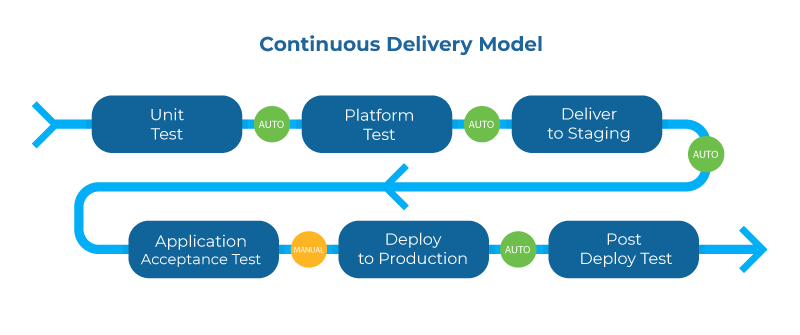
\includegraphics[scale=0.45]{img/cd.png}
    \end{figure}
    \end{frame}

\section{Vantagens da Entrega Contínua}
    \begin{frame}{Por Que Implementar Entrega Contínua?}
        \begin{itemize}
            \item Agilização dos processos;
            \item Melhoria da performace da equipe;
            \item Maior segurança e qualidade nas enregas;
            \item Aumento da satisfação dos clientes;
        \end{itemize}
    \end{frame}

\section{Implantação Contínua}
    \begin{frame}{Implantação Contínua (Continuous Deploy)}
        \begin{itemize}
            \item Melhoria da entrega contínua;
            \item Deploy em produção automatizado;
            \item Não se aplica a toda empresa;
            \item Mas deve se tentar aplicar quando possível;
            \item Deve incorporar ferramentas de monitoramento no ambiente de produção;
        \end{itemize}
    \end{frame}

\section{Continuous Delivery vs. Continuous Deploy}
    \begin{frame}{Continuous Delivery vs. Continuous Deploy}
        \begin{figure}[h]
        \centering
        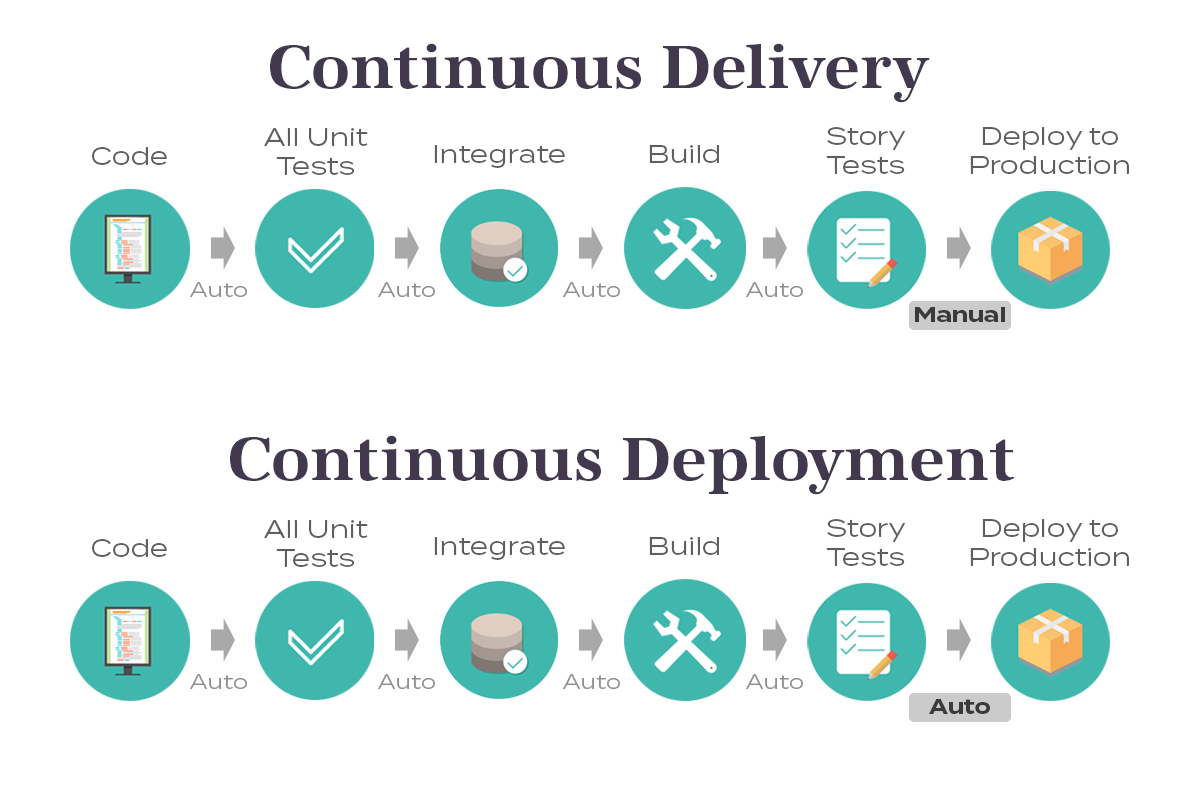
\includegraphics[scale=0.28]{img/continuous-delivery-deployment.jpg}
    \end{figure}
    \end{frame}

\section{Ferramentas de CI \& CD}
    \begin{frame}{Ferramentas de CI \& CD}
        \begin{textblock*}{5cm}(1cm,1.5cm) % {block width} (coords)
        
\includegraphics[scale=0.3]{img/jenkins.png}
    \end{textblock*}
    
    \begin{textblock*}{5cm}(3.5cm,1.5cm) % {block width} (coords)
        
\includegraphics[scale=0.07]{img/gitlab-logo-gray-rgb.png}
    \end{textblock*}
    
    \begin{textblock*}{5cm}(9.5cm,1.5cm) % {block width} (coords)
        
\includegraphics[scale=0.18]{img/gitlab-runner-logo_2x.png}
    \end{textblock*}
    
    \begin{textblock*}{5cm}(1cm,4.2cm) % {block width} (coords)
        
\includegraphics[scale=0.26]{img/trav.png}
    \end{textblock*}
    
    \begin{textblock*}{5cm}(8cm,4.5cm) % {block width} (coords)
        
\includegraphics[scale=0.23]{img/circleci-logo-stacked-fb.png}
    \end{textblock*}
    \end{frame}
    \subsection{Jekins}
        \begin{frame}{Jenkins}
        \begin{itemize}
            \item Open Source;
            \item Escrito em Java;
            \item Tem suporte a todos os principais versionadores de código do mercado: Git, Subversion, Mercurial, etc...
            \item Diversos plugins de integração;
        \end{itemize}
        \begin{textblock*}{5cm}(9.5cm,5.5cm) % {block width} (coords)
        
\includegraphics[scale=0.28]{img/jenkins.png}
        \end{textblock*}
        \end{frame}
        \subsubsection{Interface do Jenkins}
            \begin{frame}{Interface do Jenkins}
                \begin{figure}[h]
                \centering
                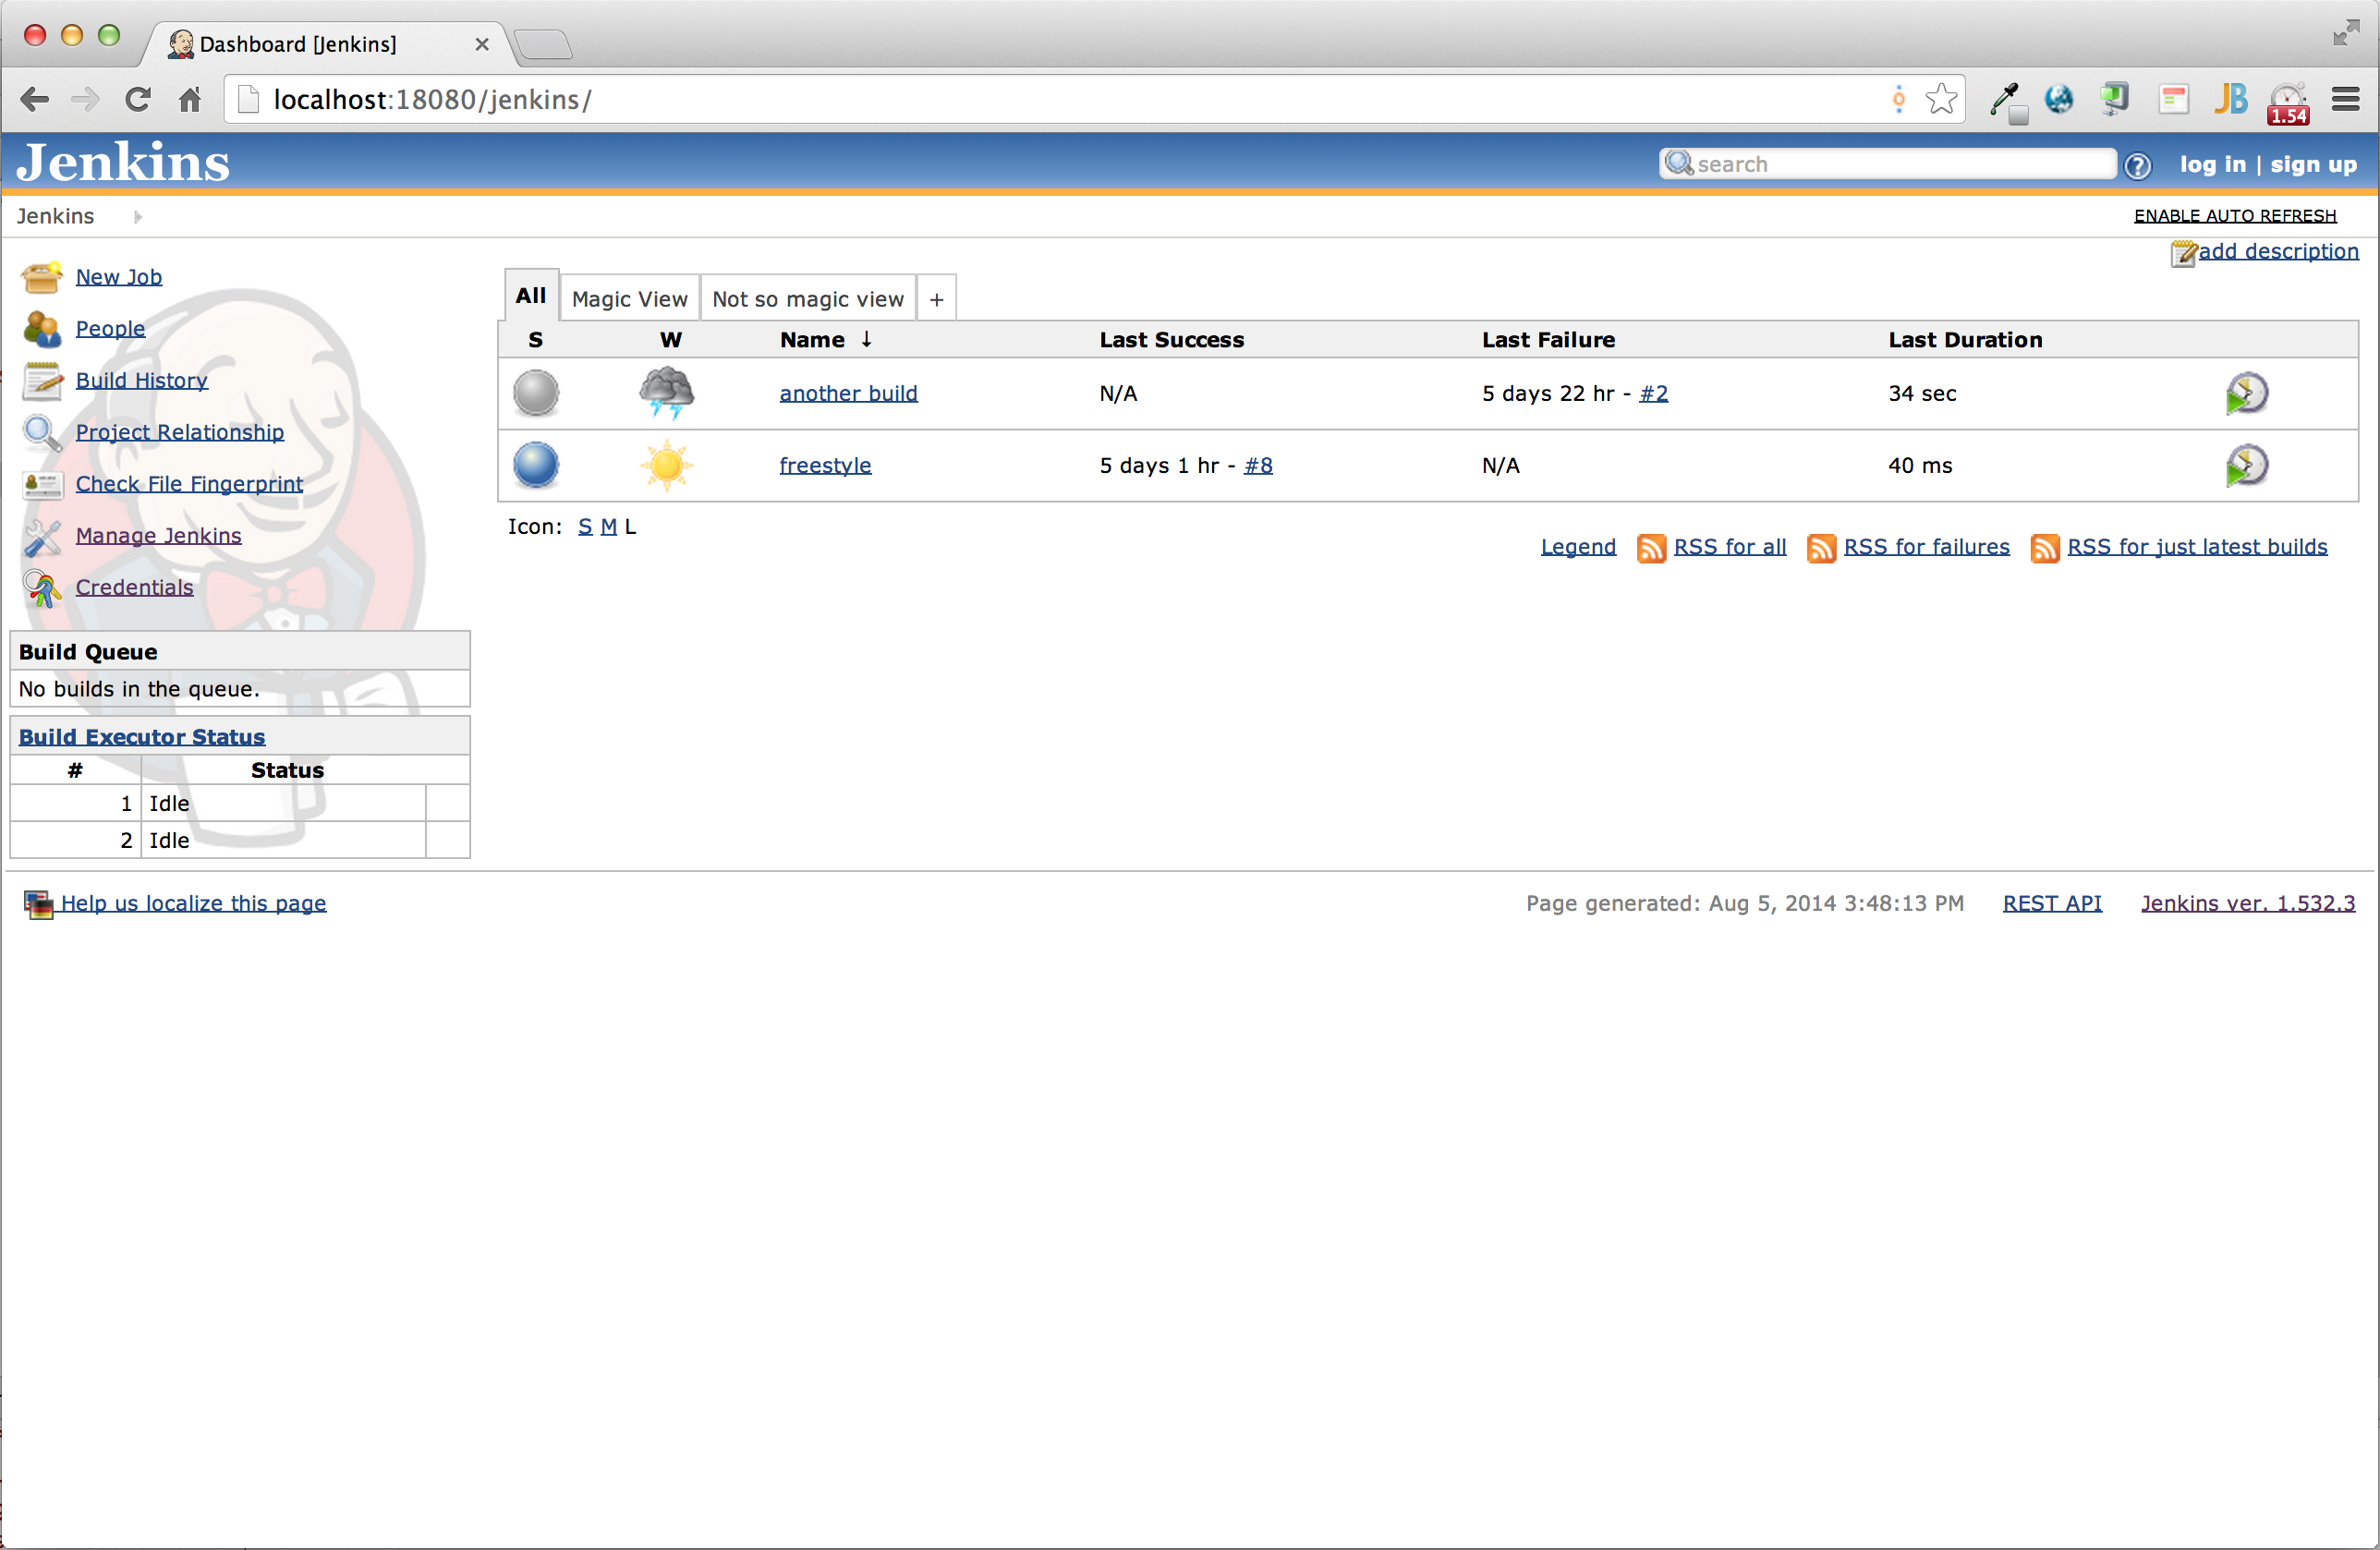
\includegraphics[scale=0.13]{img/current.png}
                \end{figure}
            \end{frame}
    \subsection{GitLab CI}
        \begin{frame}{GitLab CI}
            \begin{itemize}
                \item Proposta de manter tudo em um mesmo ambiente;
                \item Plataforma como serviço (PaaS) que permite:
                    \begin{itemize}
                        \item Commitar o seu código;
                        \item Controlar a versão e fazer code reviews;
                        \item Testes de integração;
                        \item Builds;
                        \item Deployments;
                    \end{itemize}
                \item GitLab Runner;
            \end{itemize}
        \end{frame}
    
        \begin{frame}{GitLab CI}
            \begin{figure}[h]
            \centering
            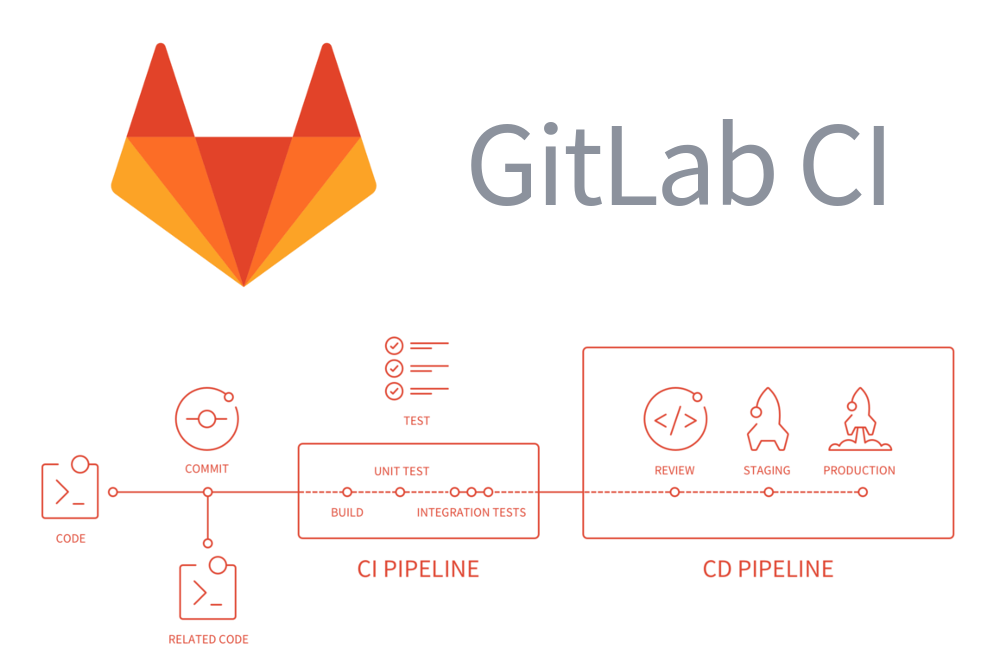
\includegraphics[scale=0.29]{img/gitlabci.png}
        \end{figure}
        \end{frame}
        
        \subsubsection{Interface do GitLab CI}
            \begin{frame}{Interface do GitLab CI}
                \begin{figure}[h]
                    \centering
                    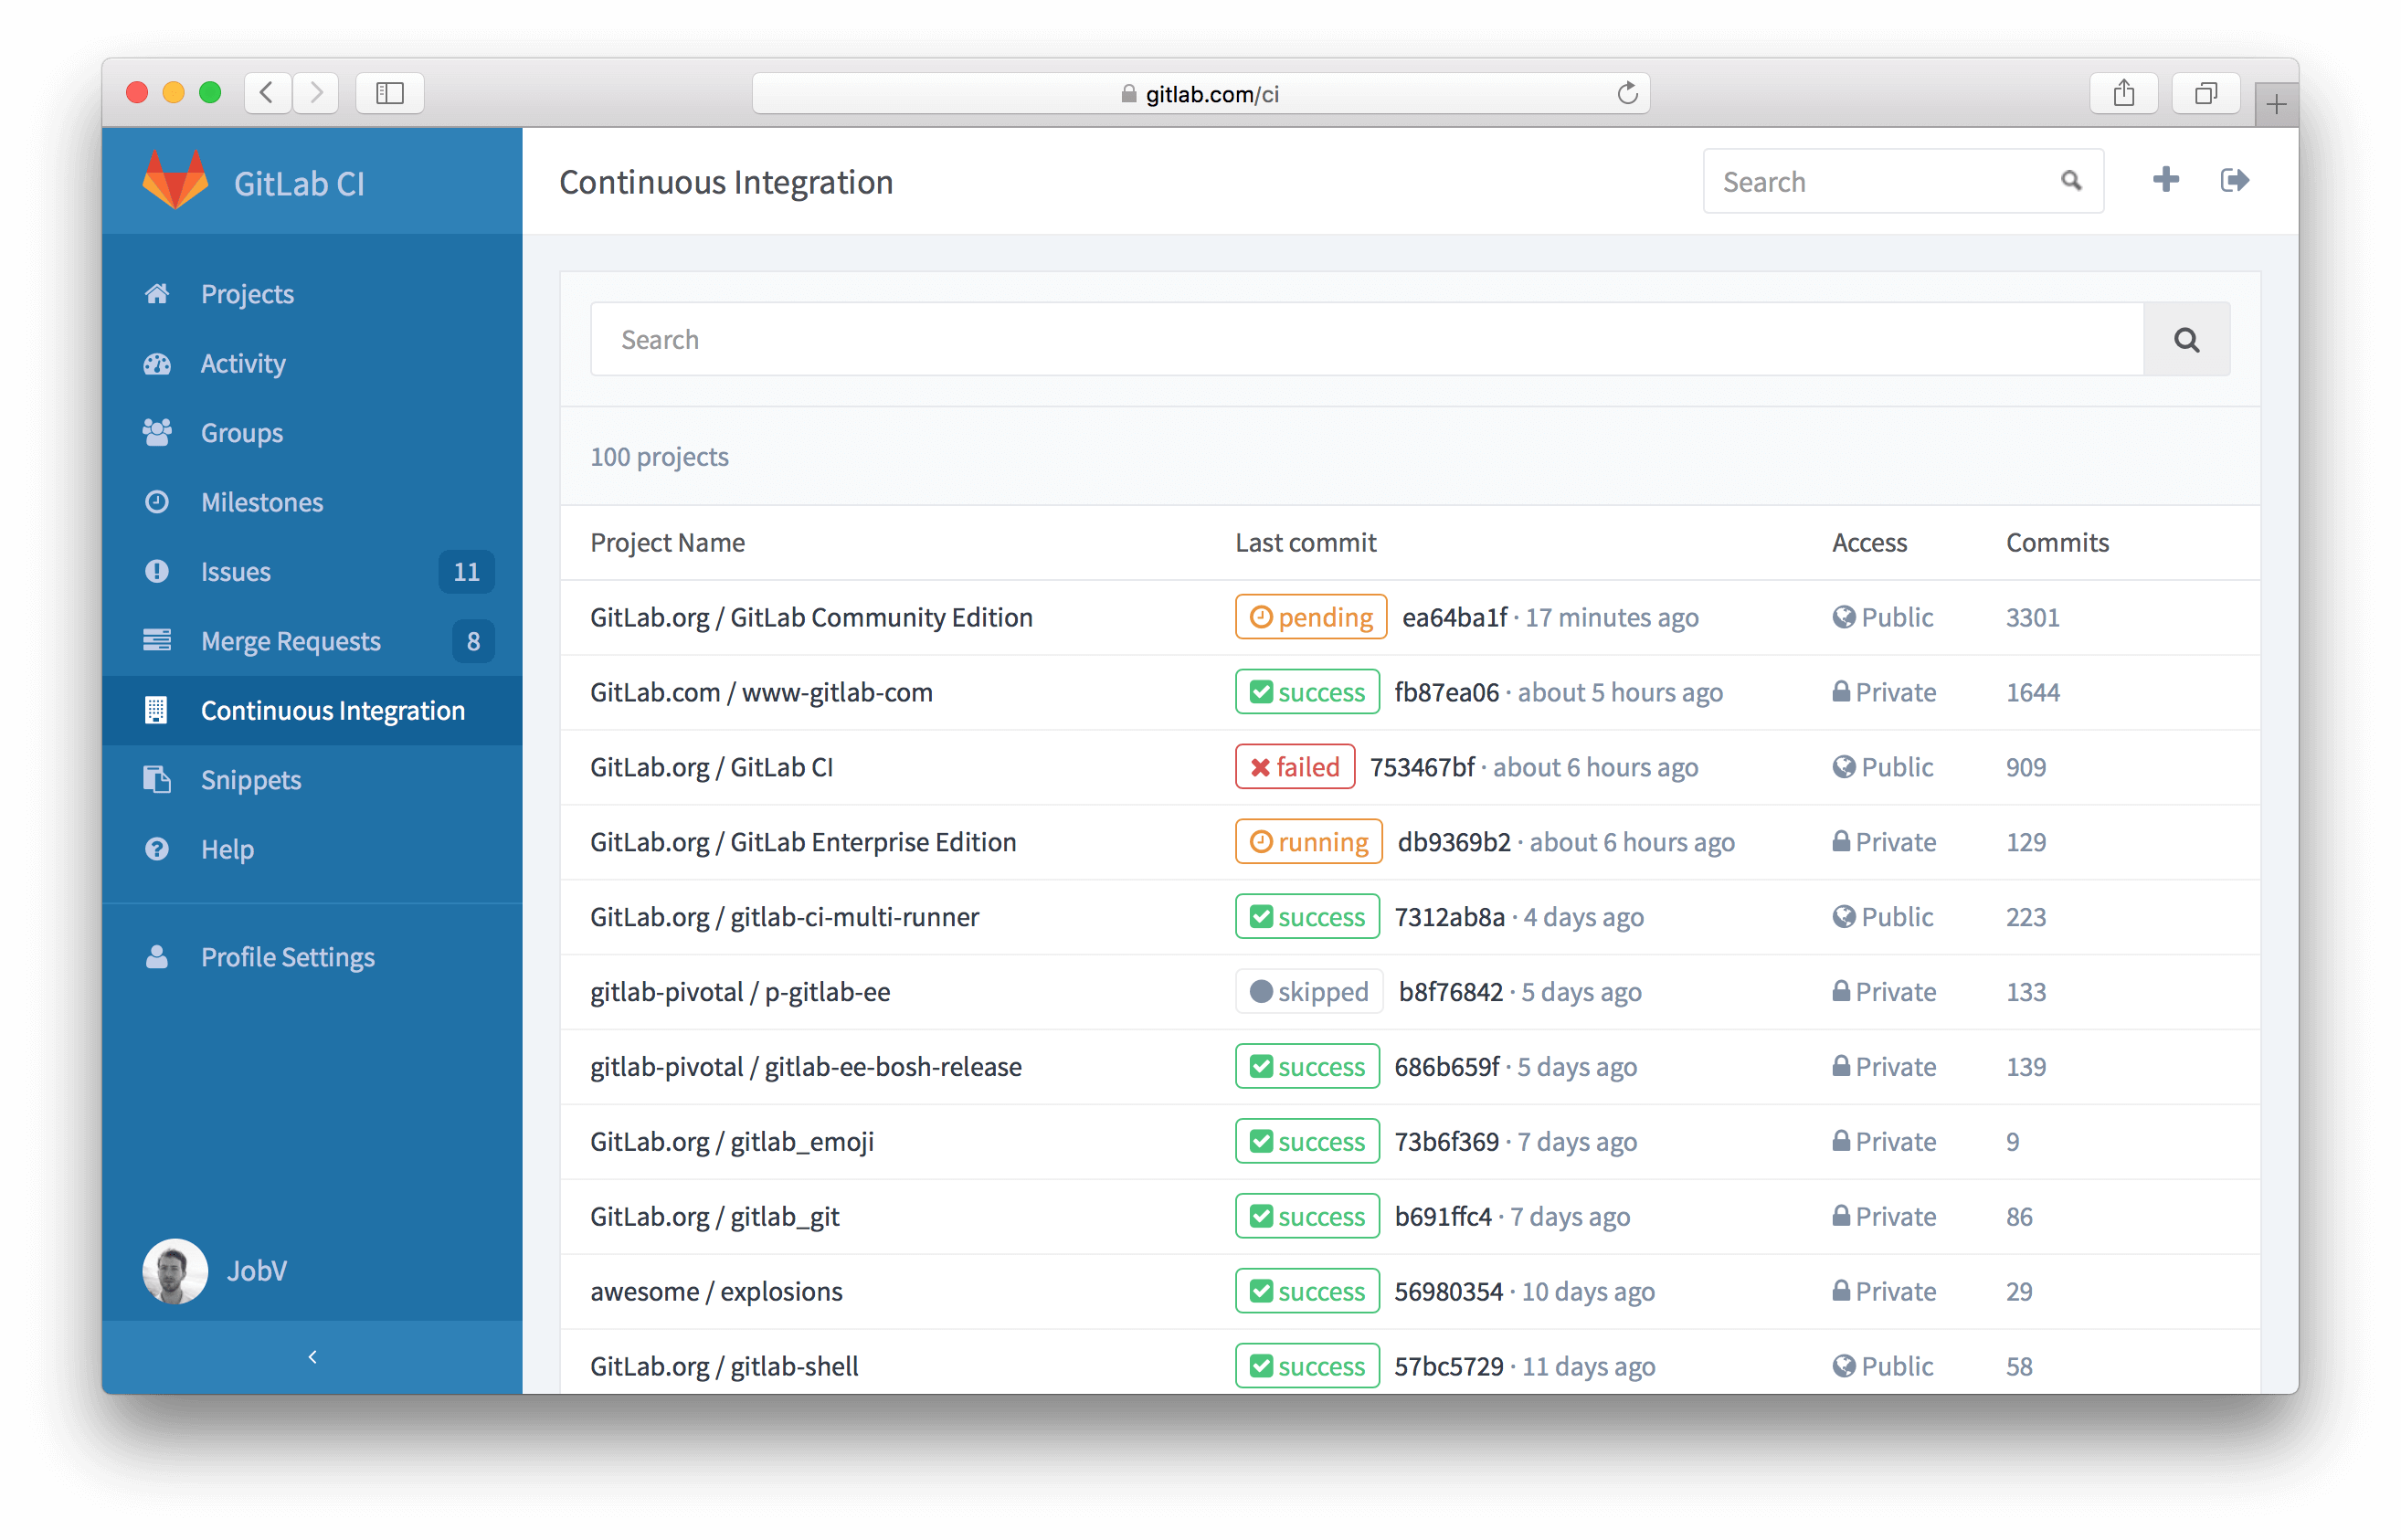
\includegraphics[scale=0.127]{img/ci_dash.png}
                \end{figure}
            \end{frame}
        
        \subsubsection{Interface do Pipeline no GitLab CI}
            \begin{frame}{Interface do Pipeline no GitLab CI}
                \begin{figure}[h]
                \centering
                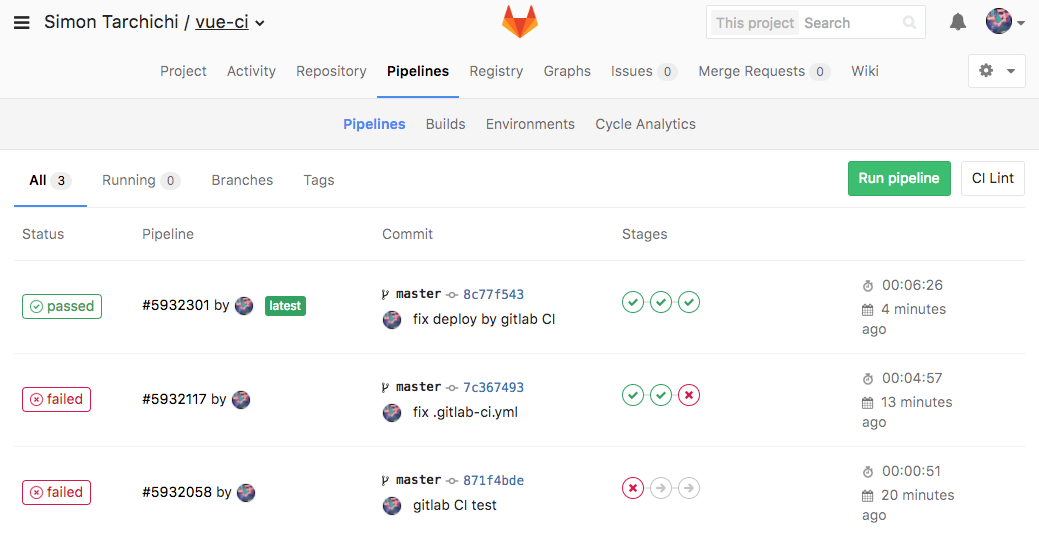
\includegraphics[scale=0.32]{img/gitlab-ci-pipelines.png}
            \end{figure}
        \end{frame}
        
\section{Conclusão}
    \begin{frame}
    \frametitle{Conclusão}
        Com uma demanda e competitividade cada vez maior, principalmente em fábricas de software, devemos nos aproveitar de aplicações e metodologias que provém ferramentas que poassam agilizar esse processo, de forma segura e rápida, com objetivo de gerar valor mais rápido e entregar um produto com qualidade para o cliente.
    \end{frame}


\begin{frame}
\begin{figure}[h]
\centering
\includegraphics[scale=0.14]{duvidas.png}
\end{figure}
\end{frame}

\section{Referências Bibliográficas}
    \begin{frame}
    \frametitle{Referências Bibliográficas}
    \begin{itemize}
    \item https://imasters.com.br/desenvolvimento/integracao-continua-vs-entrega-continua-vs-deployment-continuo
    \item https://www.4linux.com.br/diferencas-entre-integracao-deploy-e-entrega-continua
    \item https://gaea.com.br/diferencas-entre-integracao-deploy-e-entrega-continua/
    \item https://gaea.com.br/por-que-entrega-continua-e-importante-para-sua-empresa/
    \item https://www.redhat.com/pt-br/topics/devops/what-is-ci-cd
    \item https://onebitcode.com/ferramentas-devops/
    \end{itemize}
    \end{frame}
    
    \begin{frame}
    \frametitle{Referências Bibliográficas}
    \begin{itemize}
    \item https://www.concrete.com.br/2018/02/15/conheca-o-gitlab-ci/
    \item https://www.digitalocean.com/community/tutorials/como-configurar-pipelines-de-integracao-continua-com-o-gitlab-ci-no-ubuntu-16-04-pt
    \item https://jenkins.io/
    \item https://medium.com/cwi-software/testes-automatizados-no-jenkins-recursos-plugins-e-dicas-para-aumentar-a-produtividade-1685ffa1e9db
    \item https://about.gitlab.com/product/continuous-integration/
    \end{itemize}
    \end{frame}

\end{document}